\documentclass[12pt,a4paper]{article}
\usepackage{hyperref}

\title{} 
\author{Simone Balducci, Gregorio Berselli}
\date{}

\usepackage{amsmath}
\usepackage{amsfonts}
\usepackage{amssymb}
\usepackage{amsthm}
\usepackage{braket}
\usepackage[margin=3cm]{geometry}
\usepackage{pgfplots}
\pgfplotsset{compat=1.18}
\usepackage{fancyhdr}
\usepackage{physics}
\usepackage{systeme,mathtools}
\usepackage{graphicx}
\usepackage{float}
\usepackage{relsize}
\usepackage{calligra}
\usepackage{siunitx}
\usepackage[miktex]{gnuplottex}
\usepackage{epstopdf}
\usepackage[english]{babel}
\usepackage{float}
\usepackage{tikz}
\usetikzlibrary{shapes.misc}
\usepackage[style=ieee]{biblatex}
\addbibresource{./tex/biblio.bib}

\newcommand{\R}{\Re}
\newcommand{\la}{\lambda}
\newcommand{\al}{\alpha}
\newcommand{\bd}{\textbf}
\newcommand{\lang}{\left\langle}
\newcommand{\rang}{\right\rangle}
\newcommand{\lbra}{\left\lbrace}
\newcommand{\rbra}{\right\rbrace}

\begin{document}

\maketitle

\begin{abstract}
    
\end{abstract}

\tableofcontents
\pagebreak

\section{Introduction}

\section{Fair Game hypothesis}

\subsection{Class permanence with a random network}

\section{Unfair Game hypothesis}

\section{Conclusions}

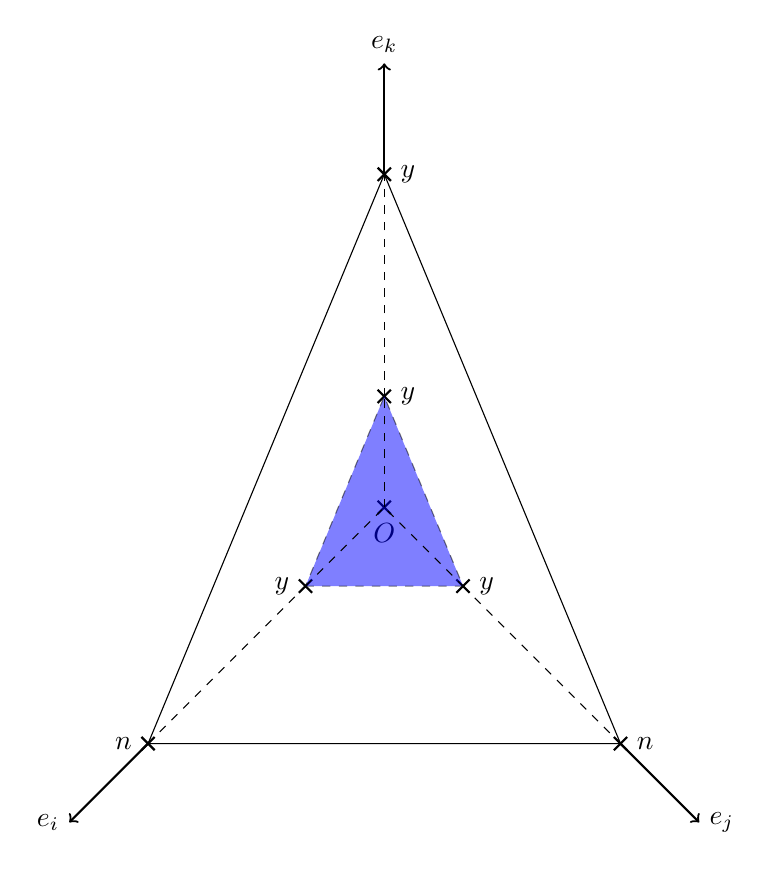
\begin{tikzpicture}
    \tikzstyle{point}=[thick,draw=black,cross out,inner sep=0pt,minimum width=4pt,minimum height=4pt]

    \node (a)[point,label={[label distance=0cm]180:$y$}] at (0,0) {};
    \node (b)[point,label={[label distance=0cm]0:$y$}] at (2,0) {};
    \node (c)[point,label={[label distance=0cm]0:$y$}] at (1,2.41) {};
    \node (d)[point,label={[label distance=0cm]270:$O$}] at (1,1) {};
    \node (e)[point,label={[label distance=0cm]180:$n$}] at (-2,-2) {};
    \node (f)[point,label={[label distance=0cm]0:$n$}] at (4,-2) {};
    \node (g)[point,label={[label distance=0cm]0:$y$}] at (1,5.23) {};
    \draw[dashed, fill=blue, opacity=0.5] (a.center) -- (b.center) -- (c.center) -- cycle;
    \draw (e.center) -- (f.center) -- (g.center) -- cycle;
    \draw[dashed] (e.center) -- (a.center);
    \draw[dashed] (b.center) -- (f.center);
    \draw[dashed] (c.center) -- (g.center);
    \draw[dashed] (a.center) -- (d.center) -- (b.center);
    \draw[dashed] (d.center) -- (c.center);

    \draw[thick, ->] (-2,-2) -- (-3,-3) node[anchor=east]{$e_i$};
    \draw[thick, ->] (4,-2) -- (5,-3) node[anchor=west]{$e_j$};
    \draw[thick, ->] (1,5.23) -- (1,6.64) node[anchor=south]{$e_k$};

\end{tikzpicture}

\printbibliography

\end{document}
